\section{FPGA}
\begin{figure}
    \centering
    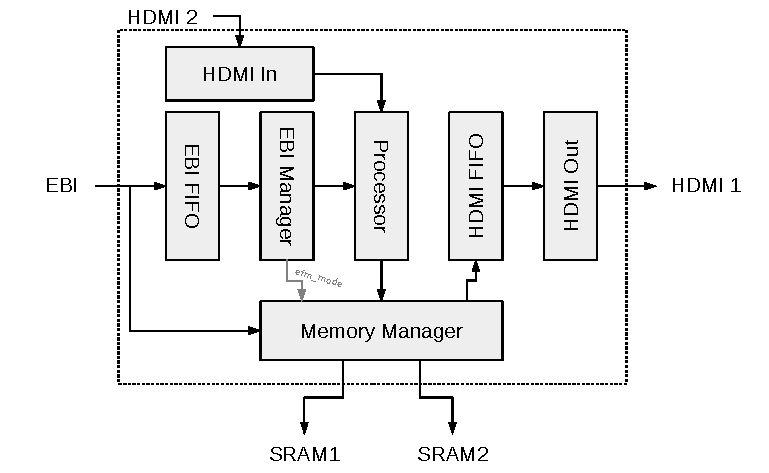
\includegraphics{img/FpgaOverview}
    \caption{FPGA Overview}
    \label{fig:FpgaOverview}
\end{figure}

The FPGA must handle an incoming video stream and the configuration data arriving from the MCU before the actual convolution is performed and the final video stream outputted. In addition, some of the different components run at different clock speeds, thus queues are needed to synchronize data on the boundaries between clock domains.

In Figure \ref{fig:FpgaOverview}, the top components on the FPGA are depicted.

\subsection{EBI}
As EBI is asynchronous, the incoming data for the FPGA must be synchronized to the processor clock domain before being used by clocked logic in the FPGA.
This is done by sending the data through a first-in first-out (FIFO) queue immediately after arrival.

After being synchronized, the EBI manager checks the addresses to determine what action to perform. In some cases, the data is resized from 16 to 24 bits and forwarded to the processor. In other cases, the data sets a control bit in the EBI manager which turns on EFM mode for the FPGA.

In EFM mode, EBI is routed to one of the memory chips to allow the MCU to read and write data and the HDMI output module is locked to the very same chip.
This allows the MCU to paint user interfaces on the screen so that the system can be controlled through buttons.
Configuration may include loading a new bit file onto the FPGA or setting up a different kernel for the processor.

\subsection{Memory}
The memory manager handles reading and writing to memory, and swapping the chips used as a double buffer when a frame is finished.
This includes calculating what addresses to place the arriving data at and what data to read.

In addition, the chip enable (or write enable) signal for the memory chips have to be pulsed in order to save data, which requires write cycle management.
This consists of a set-up phase and a write phase, giving a duty cycle of \unit[50]{\%} for the chip enable signal.

As stated in Section \ref{subsec:sram}, the memory chips are 16 bits wide, thus data from the processor must be resized from 24 bits to 16 bits before being written to memory.
Similarly, data read from the memory must be resized back to 24 bits before being sent to HDMI.

\subsection{HDMI}
Before the data from memory arrives is used by the HDMI module, it passes through a FIFO queue which has two functions:
\begin{itemize}
    \item Synchronize the data to the clock domain of the HDMI
    \item Act as a buffer in case the memory is too slow
\end{itemize}

That is, we may be able to hide the speed difference between the memory and the HDMI because there is a pause between each frame that the memory can use to catch up with the HDMI data consumption.
To make things worse, the HDMI clocks out a 24 bit pixel on each cycle while the memory only reads 16 bits each cycle.

\section{Convolution Engine}
\label{sec:processor}
In this section we will describe the processor which is at the heart of the FPGA architecture.
We will first describe the processor as a stream processor seen from the outside system before showing the inner workings.

\subsection{The Convolution Engine as a Component}
A design goal for the system was to reconfigure the FPGA depending on the task, which necessitates synthesizing several versions of the architecture so that the correct architecture may be chosen at run time.
In addition to using several architectures, each version is also programmable, allowing the kernel values, map operators and reduce operators to be programmed at runtime.
To facilitate generating different versions of the architecture we parametrized our design, allowing us to generate different architectures by simply changing a parameter once.
The parameters available are:

\begin{description}
    \item[Kernel Dimensions] \hfill \\
        The most fundamental parameter in our design, the kernel dimension dictates how many pixels we need to calculate a single output pixel.
        This is very fundamental parameter, and we will see how setting the kernel dimension will effect other important sizes in our system as we explore the system.
    \item[Image Data Input Width] \hfill \\
        The width which input image data is presented 
    \item[Pixel Width] \hfill \\
        The width of each pixel. When image input width and pixel width does not match, for instance with 16 bit input width and 24 bit pixel width, the processor must buffer and translate the input stream 
    \item[Control Data Input Width] \hfill \\
        As with input data width, the processor must know the width of the incoming control data.
    \item[Image Data Output Width] \hfill \\
        The data width that the processor should output. As with input, translating widths is necessary.
\end{description}

By parametrizing the processor we can view it as any other processor module with the inputs and outputs shown in Table \ref{tbl:ConvolutionEngineIO}.

\begin{table}[h]
    \begin{tabular}{l | l | l | l }
        &   Signal & Width\\
        \hline
        \multirow{5}{*}{Input}
        &   Image data in           & Image input width     & Data stream from camera on row format
        \\
        &   Image data valid        & 1                     & image data input is valid
        \\
        &   Control data in         & Control data width    & Data stream from MCU
        \\
        &   Control data valid      & 1                     & MCU data is valid
        \\
        &   Request image data      & 1                     & Current output data is received
        \\
        &   Reset                   & 1                     & Processor should reset
        \\\hline
        \multirow{2}{*}{Output}
        &   Image data out          & Image input width     & The processed image data on row format\\
        &   Image data valid        & 1                     & Current output data is valid
    \end{tabular}
    \caption{The interface of the processor, specified by its parameters}
    \label{tbl:ConvolutionEngineIO}
\end{table}

To the outside system the processor is now a module that once programmed operates on a data stream of an image and outputting a processed stream. 
By using valid signals the outside system can provide data at any pace, and throttle the output by requesting data when the processor indicates that data is ready. 

\subsection{Architecture of the processor}

Figure \ref{fig:conv_engine} shows the top level schematic of the processor with the following components:

\begin{description}
    \item[Input and output buffers] \hfill\\
        The input buffer is a double buffer resonsible for buffering rows of image data and feed it to the processor.
        The buffer holds several rows of image data, and when it is full it feeds data to the processor as a series of column slices while the other buffer is filled.\\
        The output buffer retrieves data from the processor as a series of column slices and rearranges the output back to row format.
        Figure \ref{fig:sweep_feed} shows how the input buffer feeds the processor with data from a buffered set of rows.
        When data is fed on a column major format within its set of rows we call the data stream a \textit{sweep}, inspired by the way a window is washed by sweeping it with a squeegee.
        The column slices in the sweep are called \textit{sweep columns}.
    \item[Control] \hfill\\
        The control unit is responsible for keeping track of the input and output buffers, waking the processor once an input buffer is ready and making sure the output buffer is empty before a new feeding cycle is started.
        The control unit is also responsible for programming the processor after a reset.
    \item[Processor] \hfill\\
        The heart of the convolution design, where the actual convolution happens
\end{description}

The processor does the following tasks:
\begin{itemize}
    \item Provide a clean interface to the outside system, accepting an image stream and providing an output stream on row major format, adding tolerance for input streams which may come at uneven intervals. 
    \item Once the input buffer is ready, wake up the core and provide data as an uninterrupted column major image stream, essentially working as a wrapper for the core.
\end{itemize}

Having established how the processor provides an interface for the core, we will now see how the core works internally.

\begin{figure}[h!]
    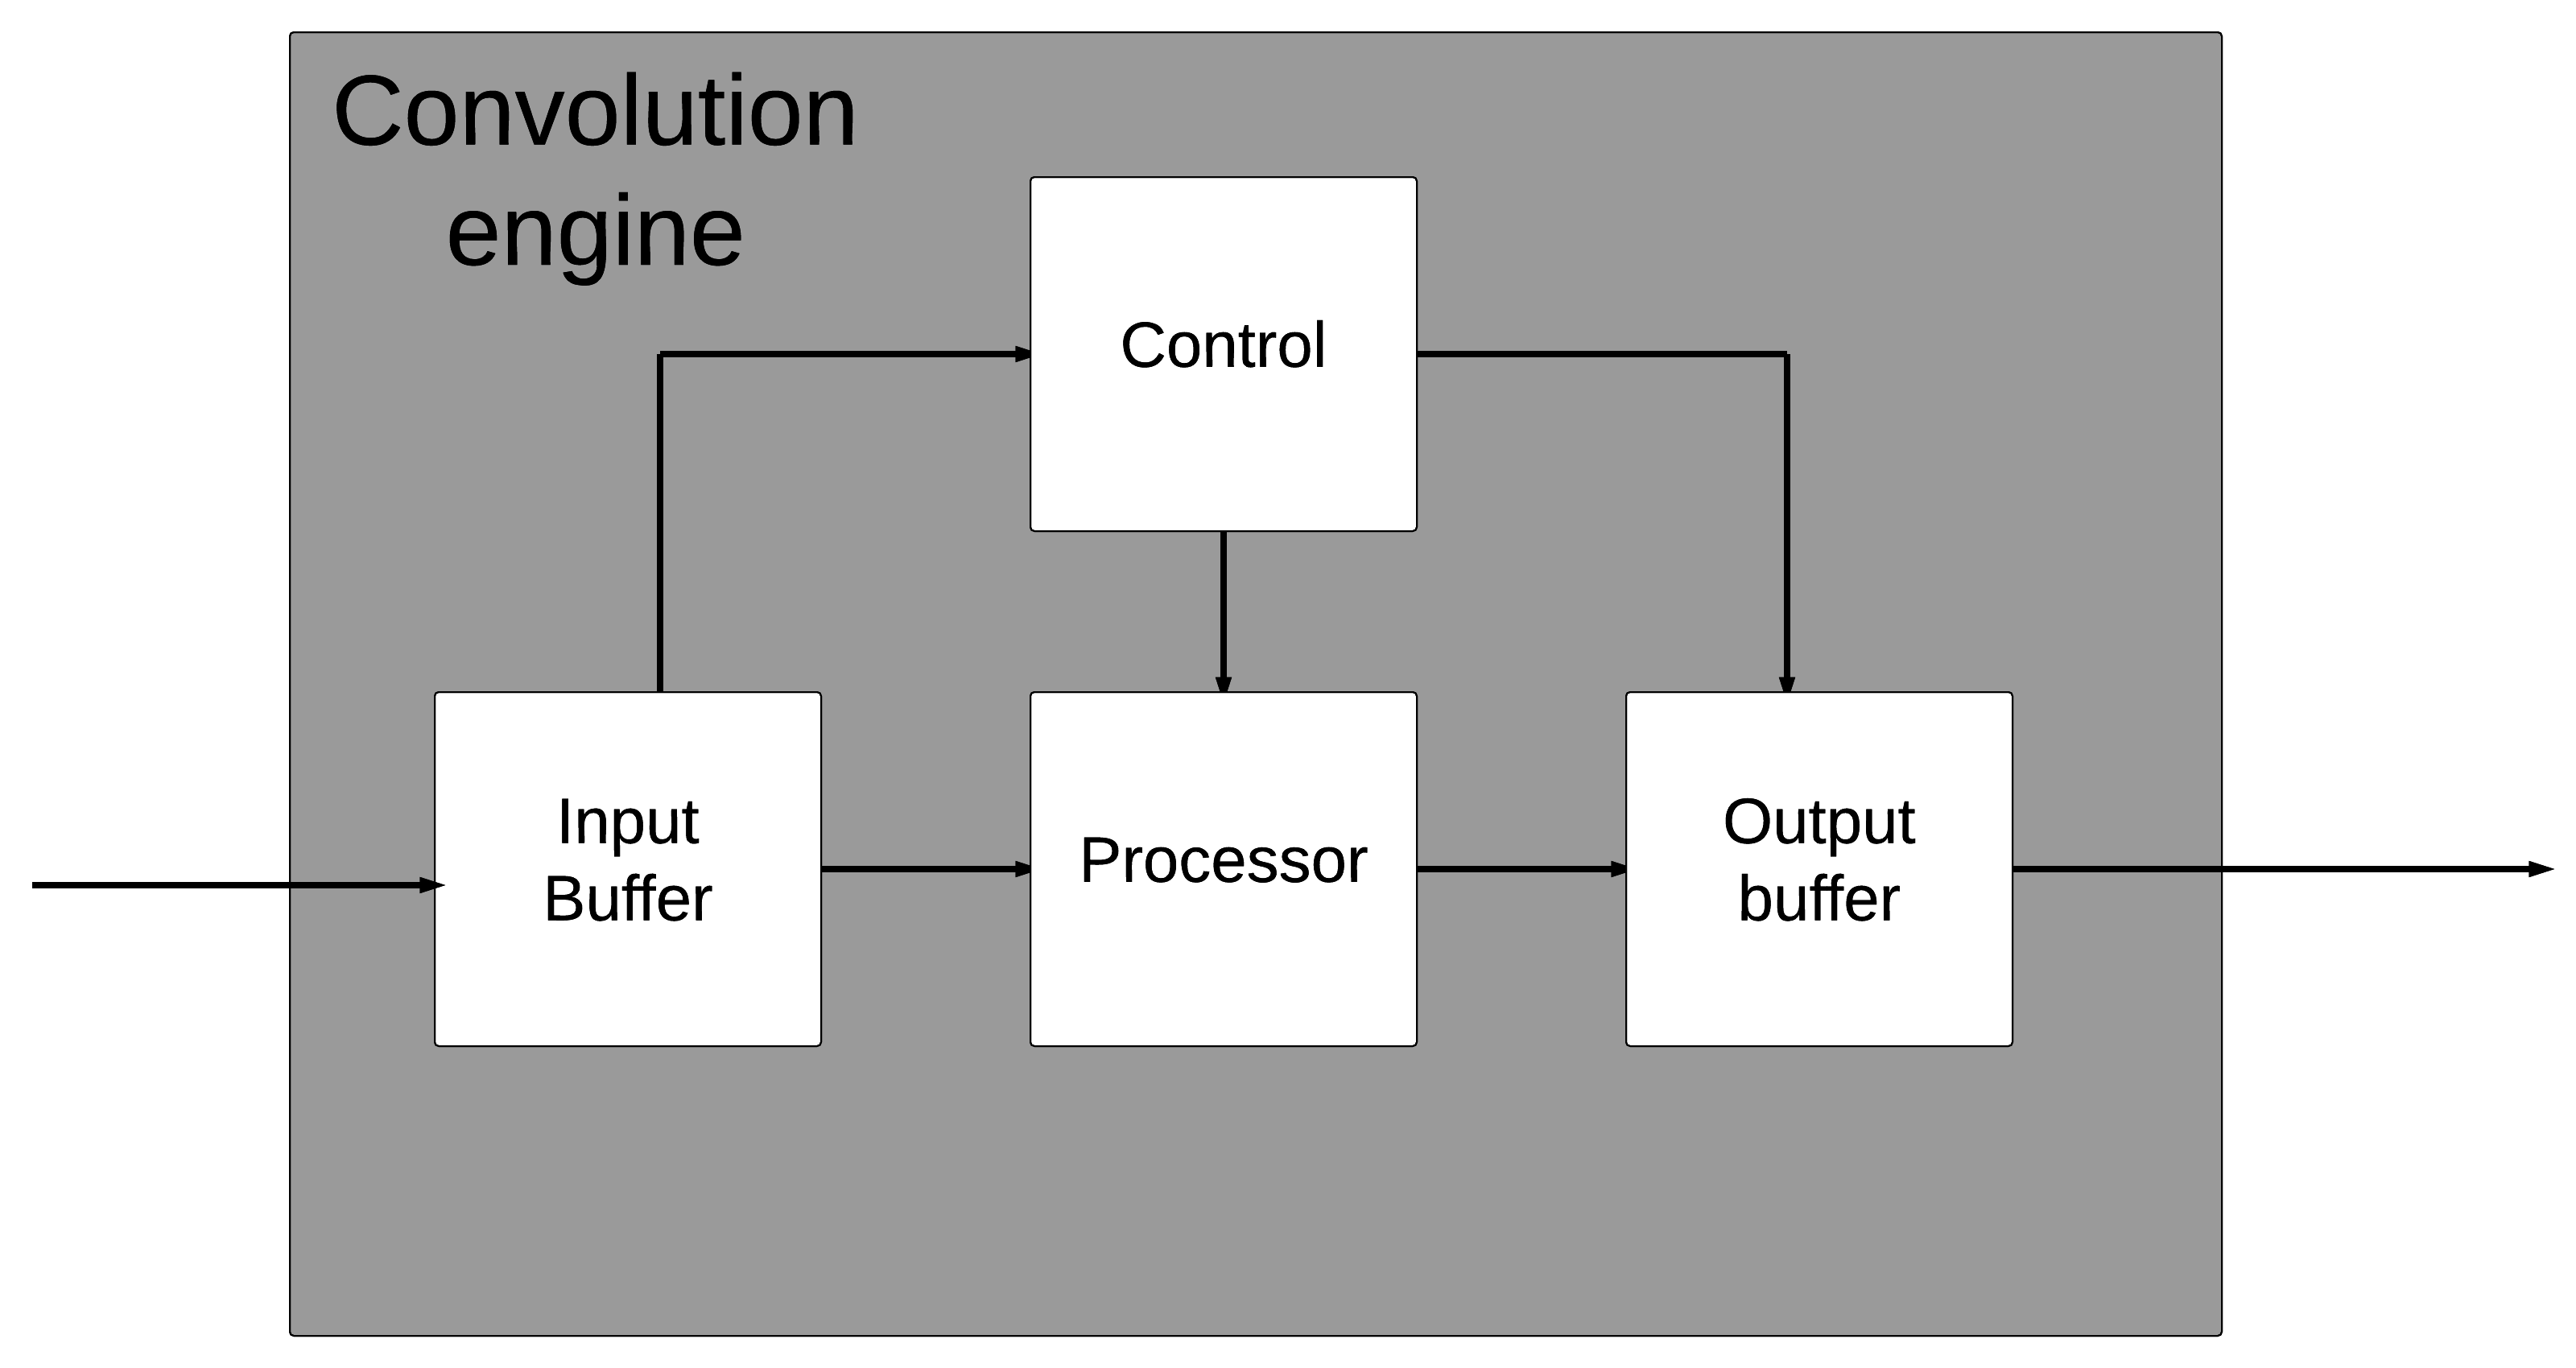
\includegraphics[width=\linewidth]{img/convolution_engine.png}
    \caption{The top level schematic of the processor.}
    \label{fig:conv_engine}
\end{figure}

\subsection{Core}
This section provides a description of the heart of our architecture.
Figure \ref{fig:convolution_processor} shows an overview of the core which contains four modules:
To illustrate how the components work we describe how the first frame of a videostream is processed.

\begin{figure}[h!]
    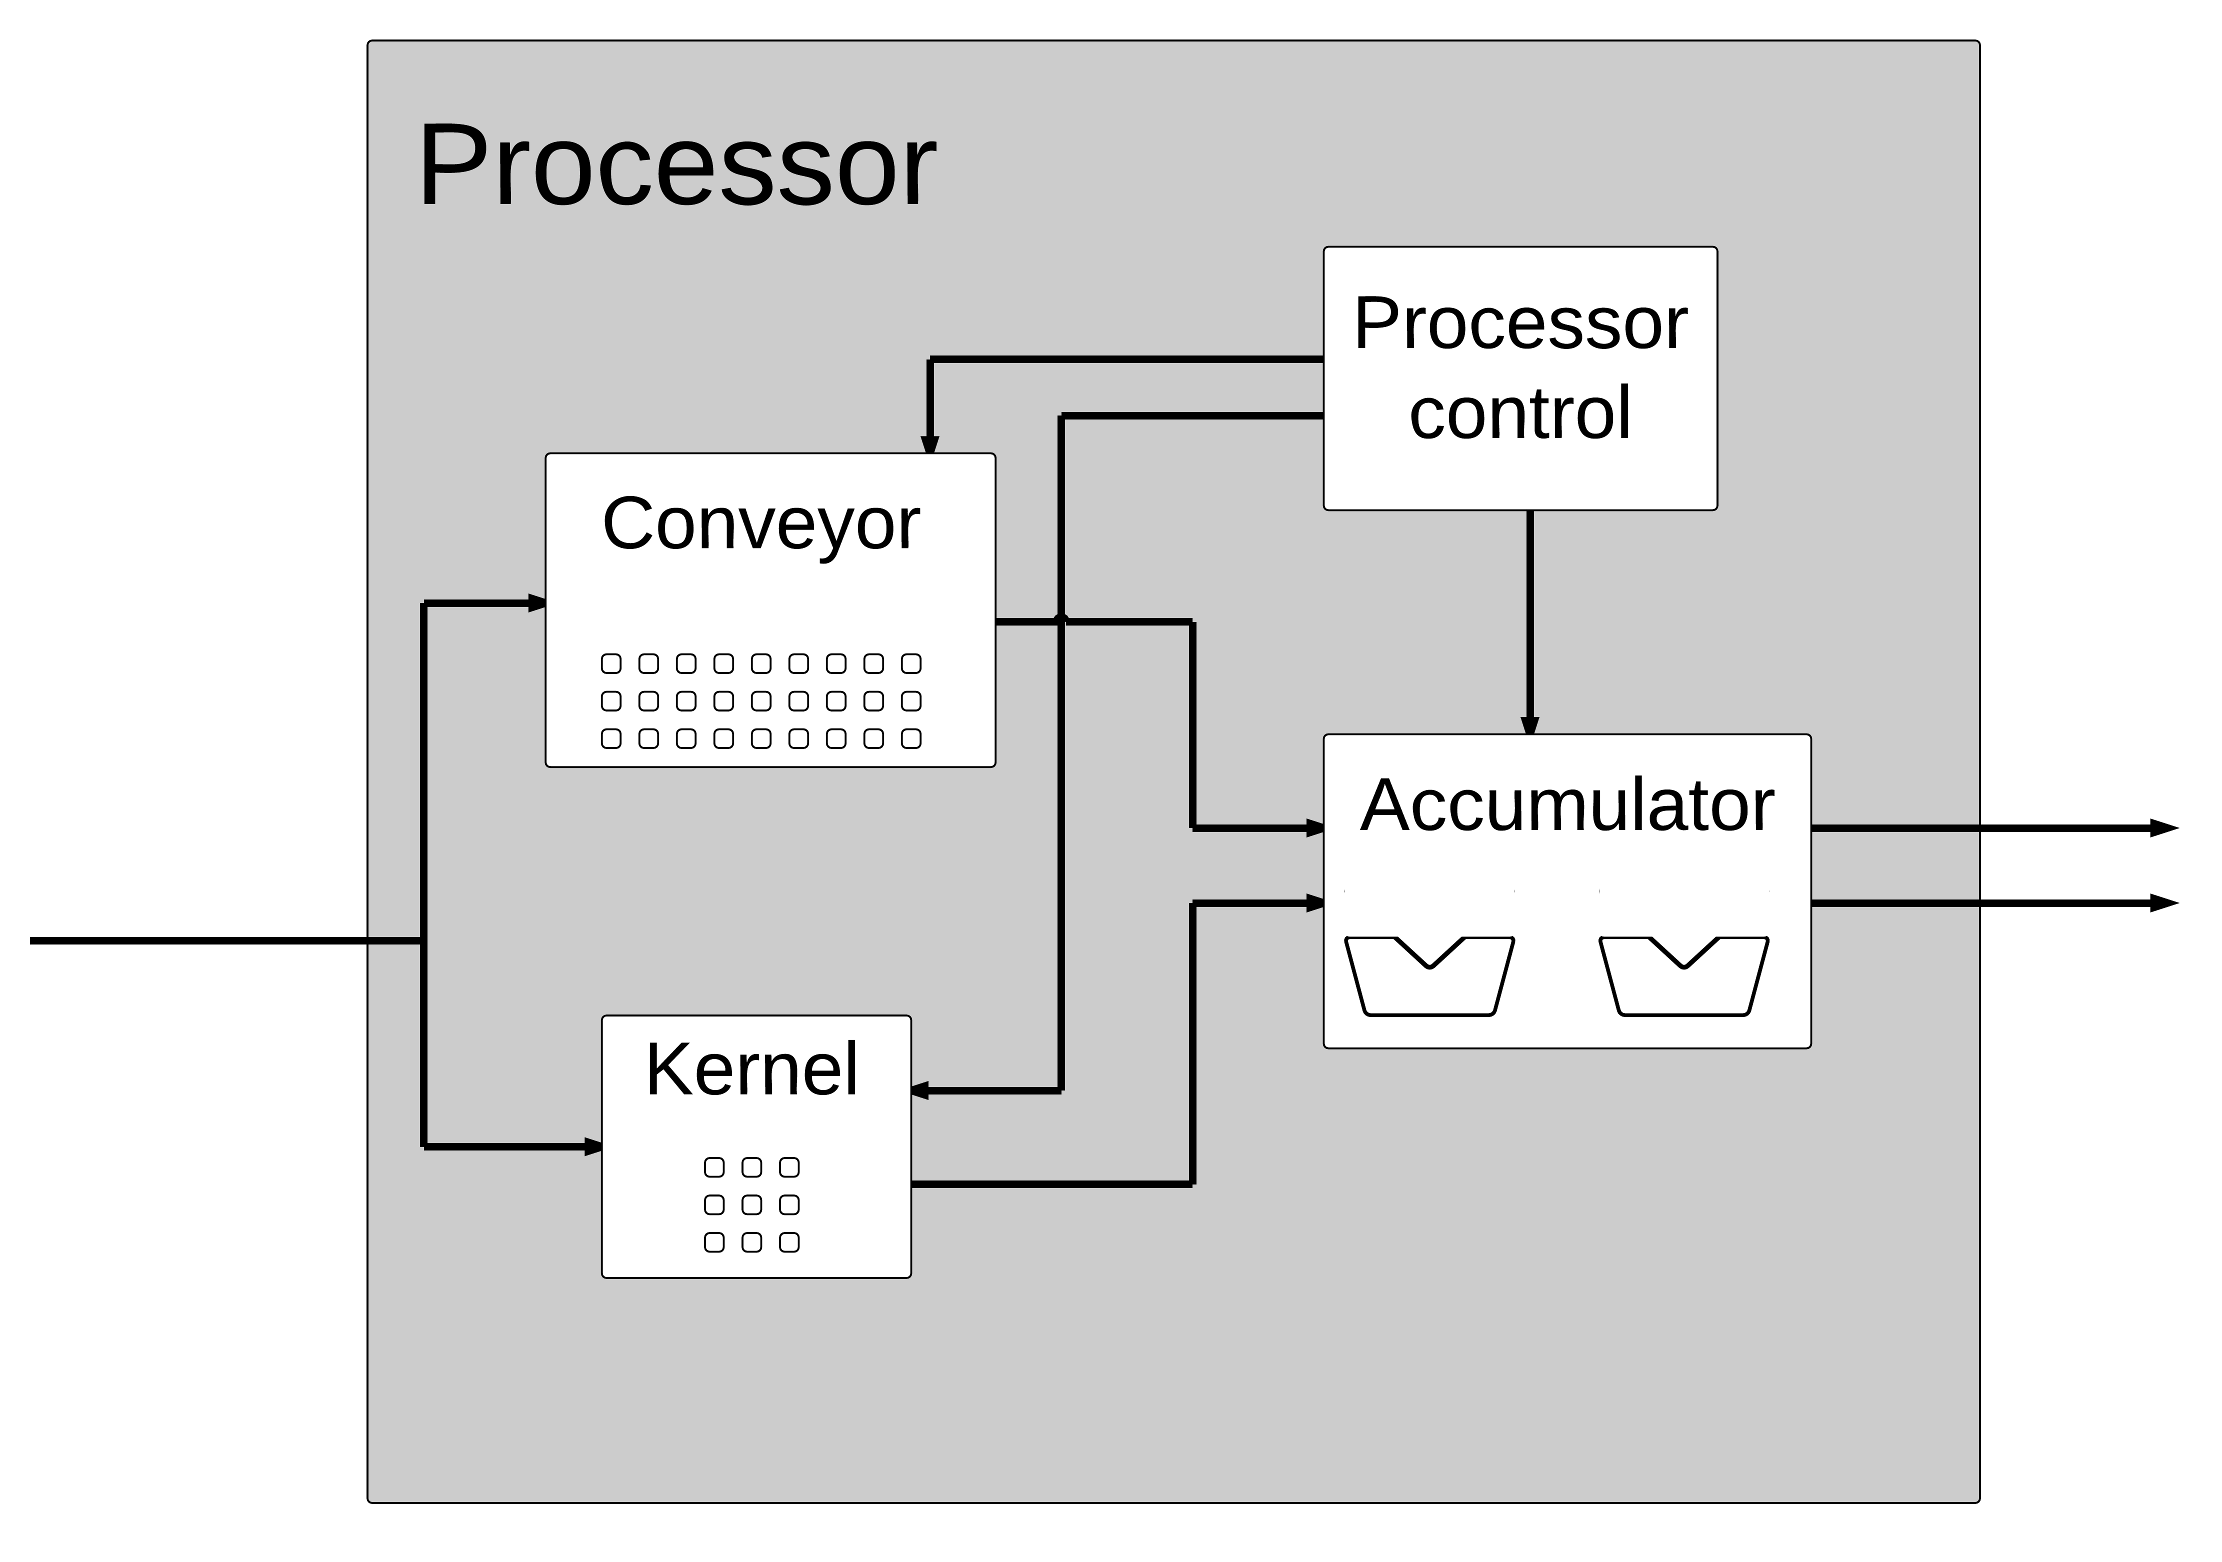
\includegraphics[width=\linewidth]{img/processor_small.png}
    \caption{The four main components of the core.}
    \label{fig:convolution_processor}
\end{figure}

From the outside, the core is a module working on sweep slices as shown in \ref{fig:sweep_feed}.
A good analogy for how the image is processed is how a window cleaner washes a window.
If we let the dirty window be our original picture, and the clean image be the processed image, the process of convolution is akin to sweeping the squeegee over the window horizontally.
In our analogy, a very small part of the window is under the squeegee at any time.
Similarily, our core works on a small part of the image at any time, only large enough to contain enough pixels to calculate a single slice of output pixels, called the \textit{sweep frontier}, as shown in figures \ref{fig:frontier1} and \ref{fig:frontier2}.
To illustrate how data is fed we can view each row in the sweep as a stack.
The rows then take turns popping one of its elements such that the core effectively gets column slices.
The core consists of the following components:

\begin{description}
    \item[Conveyor] \hfill\\ 
        The conveyor is a special register file consisting of several rows of pixel registers, which holds the pixels currently in the sweep frontier.
        Data is delivered to the accumulator in a pattern controlled by the control unit, it is however never explicitly requested.
    \item[Kernel Buffer] \hfill\\
        The kernel buffer maintains the kernel data and must provide the correct kernel data for each map operation performed in the accumulators.
        This module is also responsible for programming operators.
    \item[Accumulator] \hfill\\
        To convolute a pixel, we need one mapping unit which maps the neighbourhood of a pixel in sequence, and one reduction unit which performs a reduce operation with the input from its associated mapping unit, and a partially processed pixel.
        Together these two units forms a single accumulation unit, and by employing a row of these units together we can compute several pixels in parallel.
        The accumulator consists of a row of these functional units working on pixels in parallel.
    \item[Control Unit] \hfill\\
        In order for the accumulators and pixel conveyor to be in sync a control unit sends control signals periodically, which are then propogated throughout the system.
\end{description}

Figure \ref{fig:convolution_processor} shows the insides of the core. 
The conveyor belt shows three rows, each row keeping a column slice from the sweep frontier shown in \ref{fig:frontier1} and \ref{fig:frontier2}.
We will now explore each part of the core in greater detail.

\subsubsection{Conveyor}
The conveyor maintains the sweep frontier, and feeds pixel data to the accumulators.
It consists of a grid of pixel registers, each row holding a sweep slice.
Since each pixel in a slice corresponds to a different row, every pixel register in a row has a one to one correspondence to one of the rows of the sweep currently feeding the core.
To reiterate on this, a row in the conveyor corresponds to one of the slices in the input buffer, not a row in the input image.
Data management on the conveyor is done by sending keys which are are issued from the control unit, and passed from register to register within a row.
At any time, there is on each row two keys held by different registers: a read key and a write key.
When holding a write key the register is write enabled and should read data from the row above it, while a read key tells the register that its content should be driven its content to an interconnect which the accumulator and the row below it can read from.
Input to the conveyor is available to the entire top row, so in order to ensure that only the corresponding pixel register reads the data, the control module has to issue a key to the row at the right time.
To illustrate, in \ref{tbl:timing1} and \ref{tbl:timing2} we show when each row has access to a read key for a 3x3 kernel:
\begin{table}[h]
    \begin{tabular}{l*{16}{c}r}
    Time (cycle)        & $T_{0}$ & $T_{1}$ & $T_{2}$ & $T_{2}$ & $T_{4}$  & $T_{5}$ & $T_{6}$ & $T_{7}$ & $T_{8}$ & $T_{9}$ & $T_{10}$ & $T_{11}$ & $T_{12}$ & $T_{13}$ & $T_{14}$\\
    \hline
    Row 1                   & 4 & 5 & 6 & 7 & 8 & 9 & \cellcolor{gray75} 1 & \cellcolor{gray75} 2 & \cellcolor{gray75} 3 & 4 & 5 & 6 & 7 & 8 & 9 & \\
    Row 2                   & 7 & 8 & 9 & \cellcolor{gray75} 1 & \cellcolor{gray75} 2 & \cellcolor{gray75} 3 & 4 & 5 & 6 & 7 & 8 & 9 & \cellcolor{gray75} 1 & \cellcolor{gray75} 2 & \cellcolor{gray75} 3 & \\
    Row 3                   & \cellcolor{gray75} 1 & \cellcolor{gray75} 2 & \cellcolor{gray75} 3 & 4 & 5 & 6 & 7 & 8 & 9 & \cellcolor{gray75} 1 & \cellcolor{gray75} 2 & \cellcolor{gray75} 3 & 4 & 5 & 6 & \\
    \end{tabular}
    \caption{A sequence diagram showing which registers in each row is being read at each timestep. Greyed out cells shows the pixels in the neighbourhood of the output pixel corresponding to output row 1}
    \label{tbl:timing1}
\end{table}
\\ \\
\begin{table}[h]
    \begin{tabular}{l*{16}{c}r}
            Time (cycle)        & $T_{0}$ & $T_{1}$ & $T_{2}$ & $T_{2}$ & $T_{4}$  & $T_{5}$ & $T_{6}$ & $T_{7}$ & $T_{8}$ & $T_{9}$ & $T_{10}$ & $T_{11}$ & $T_{12}$ & $T_{13}$ & $T_{14}$\\
        \hline
        Row 1                   & \cellcolor{gray75} 4 & 5 & 6 & 7 & 8 & 9 & 1 & \cellcolor{gray75} 2 & \cellcolor{gray75} 3 & 4\cellcolor{gray75} & 5 & 6 & 7 & 8 & 9 & \\
        Row 2                   & 7 & 8 & 9 & 1 & \cellcolor{gray75} 2 & \cellcolor{gray75} 3 & \cellcolor{gray75}4 & 5 & 6 & 7 & 8 & 9 & 1 & \cellcolor{gray75} 2 & \cellcolor{gray75} 3 & \\
        Row 3                   & 1 & \cellcolor{gray75} 2 & \cellcolor{gray75} 3 & 4\cellcolor{gray75} & 5 & 6 & 7 & 8 & 9 & 1 & \cellcolor{gray75} 2 & \cellcolor{gray75} 3 & 4\cellcolor{gray75} & 5 & 6 & \\
    \end{tabular}
    \caption{A sequence diagram showing which registers in each row is being read at each timestep. Greyed out cells shows the pixels in the neighbourhood of the output pixel corresponding to output row 1}
    \label{tbl:timing2}
\end{table}
\\ \\
We see that the second leftmost output pixel follows the same pattern, only shifted left by one cycle.
A register is given a read key not only to make its content available to the accumulators, but also so that the row below may have its content written to it in order to propagate data downwards.
Each register should read the register directly above, so the write keys must be issued such that a register only has write enabled when the register above it is currently driving the interconnect.
For our conceptual design, this is easy, however in the actual implementation we move data using register balanced multiplexer trees rather than simply driving a bus.
This means a write key is not really given to the register, but to a multiplexer deciding which register should currently be read.
Additionally we use a secondary write key since the mux tree has two stages, but we will not elaborate further on this since it adds unescessary detail.

\subsubsection{Accumulator}
As each pixel register in the conveyor corresponds to a row in the sweep, each accumulation unit corresponds to an output pixel.
For a 3x3 kernel each sweep consists of 9 rows, which provides 7 output rows since the top and bottom row of each sweep misses some of its neighbours.
Each accumulation unit corresponds to one output row, and we thus have 7 accumulation units.\\
Conversely, for a 5x5 convolution kernel we would use 25 input rows, and lose two rows in each end from missing neighbours, resulting in 21 output rows, and 21 accumulation units.
From the table in the conveyor section, we see that each accumulation unit can map all the necessary pixels by correctly timing which row to read from.
In the case of the first accumulator, it should read from row 3 at time $T0, T1$ and $T2$, row 2 at time $T3, T4$ and $T5$, and row 1 at time $T6, T7$ and $T8$, as shown in grey.
At $T8$ all necessary pixel data is read, and the accumulated result is output and a new cycle begins.
The second table in the conveyor section shows the same pattern for the accumulator corresponding to output row 2, only delayed by one cycle.
This delay means that every accumulator can access the data it needs by simply timing when it reads output from the rows.
Additionally, since each accumulator is delayed one cycle relative to its neighbour, the access patter for kernel values is similarily delayed.
This kernel access pattern means every accumulator needs the kernel used by its predecessor last cycle, meaning that rather than keeping kernels in a central repository we can keep them in a shift register with each element very close to an accumulator.
Rather than keeping track of their progress, each accumulator passes a special flush key akin to how registers use read and write keys. Upon recieving a flush key an accumulation unit resets its content and its finished data is written on the output wire.

\subsubsection{The Control unit}
The control unit is responsible for issuing keys to the rows at periodic intervals such that reads, writes, flushing and selecting accumulator output is correctly synchronized.
In addition to synchronizing the accumulators and conveyor, the control unit puts the core to sleep when no data is available, and is responsible for sending signals indicating that the accumulators should read instruction data.
The issuing of keys is done by a simple state machine, for which the logic can be calculated at synthesiz time, since it is dependant on kernel size alone. 

\subsubsection{Kernel buffer}
The kernel buffer is responsible for collecting kernel data at programming time, and to supply the correct kernel at the correct time to the mapping unit.
In figure \ref{fig:convolution_processor} we show the kernel buffer holding all the kernels in a separate buffer, but as described in the accumulator section this buffer is actually a chained set of registers where each register is close to one of the accumulation units.
When in programming mode, the kernel buffer gets instructions from the pixel stream rather than a separate channel.
First, instructions are sent, which are then sent as kernels to the mappers instead of using a separate instruction channel.
When piggybacking instructions on the kernel chain, we need to wait for the instructions to fully propagate, but this is an acceptable delay since programming is done only once per run.
In addition to providing instructions, the kernel buffer is also responsible for realigning kernels when the core goes to sleep, such that when a new feed cycle begins the system is in the state that the control state machine expects.


\begin{figure}[h!]
    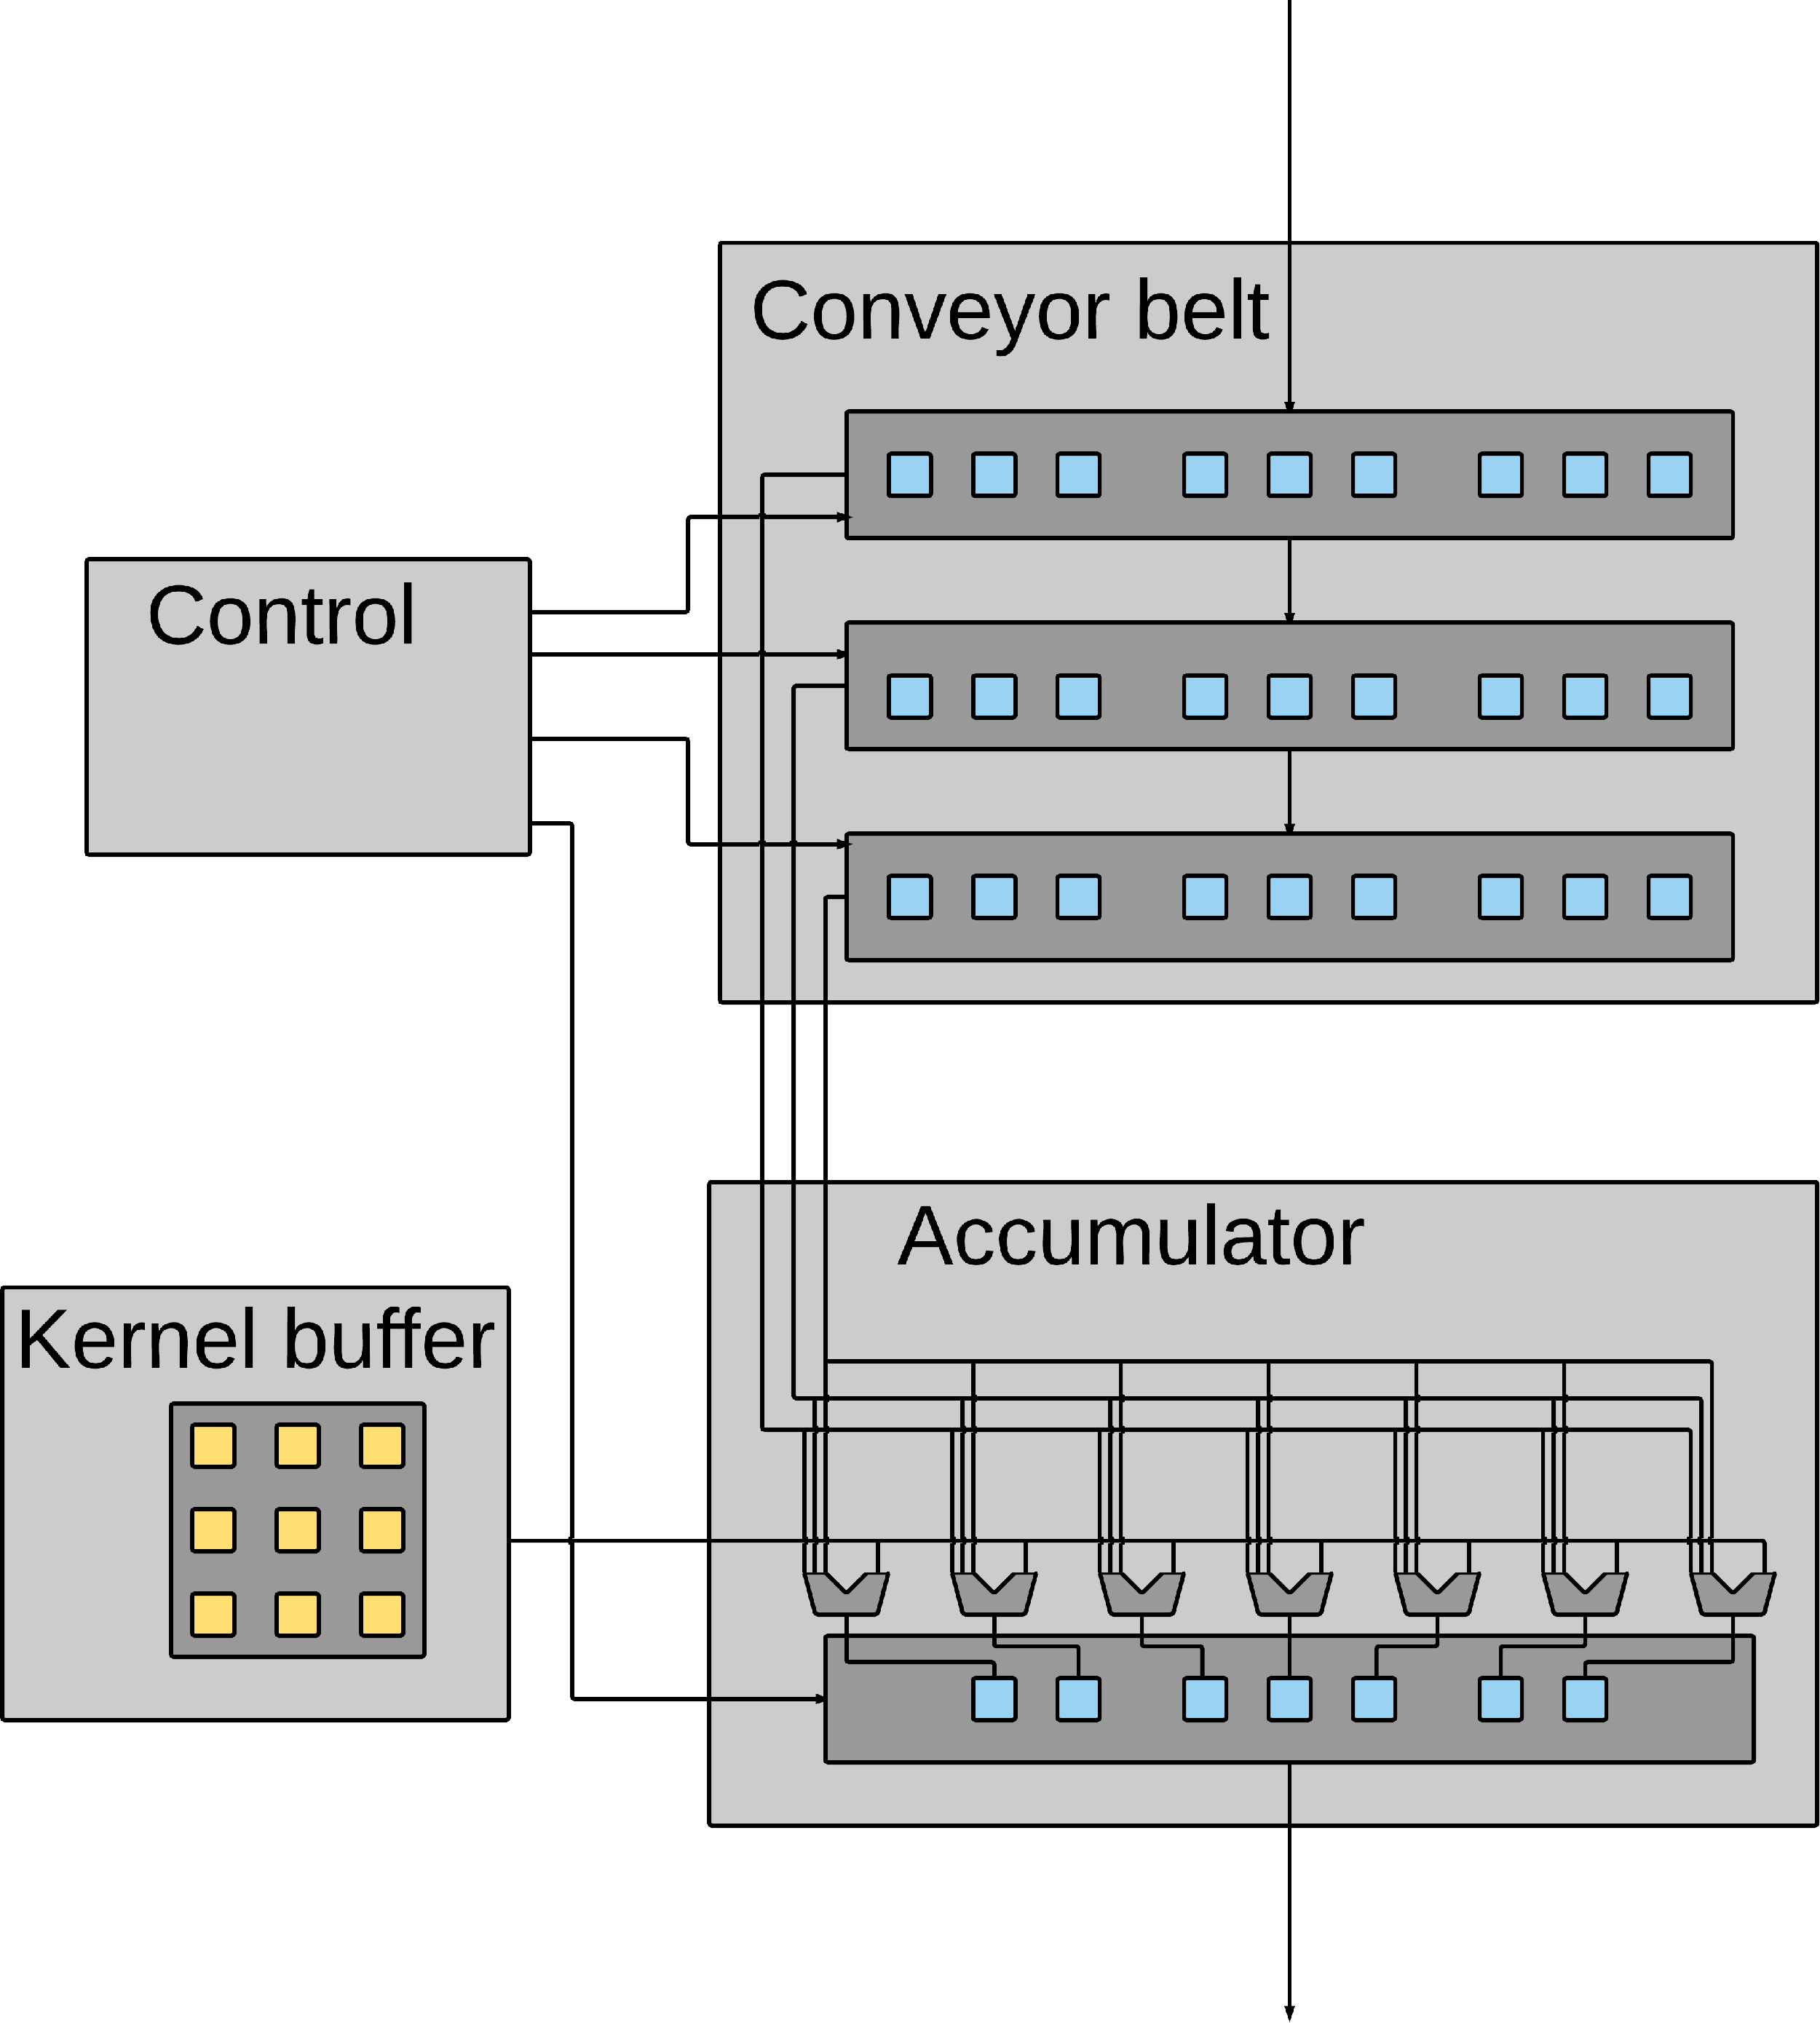
\includegraphics[width=\linewidth]{img/processor_overview_small.png}
    \caption{The four core units in the convolution process.}
    \label{fig:processor_core}
\end{figure}

\begin{figure}[h!]
    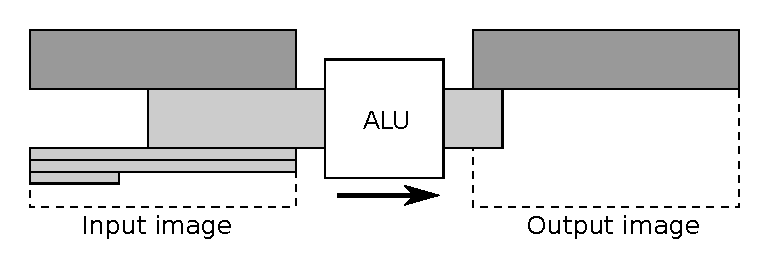
\includegraphics[width=\linewidth]{img/daisy_processing.pdf}
    \caption[Buffering and feeding of sweeps.]{A full sweep has been buffered, and is being fed to the processor. Meanwhile a new sweep is being buffered}
    \label{fig:sweep_feed}
\end{figure}

\begin{figure}[h!]
    \centering
    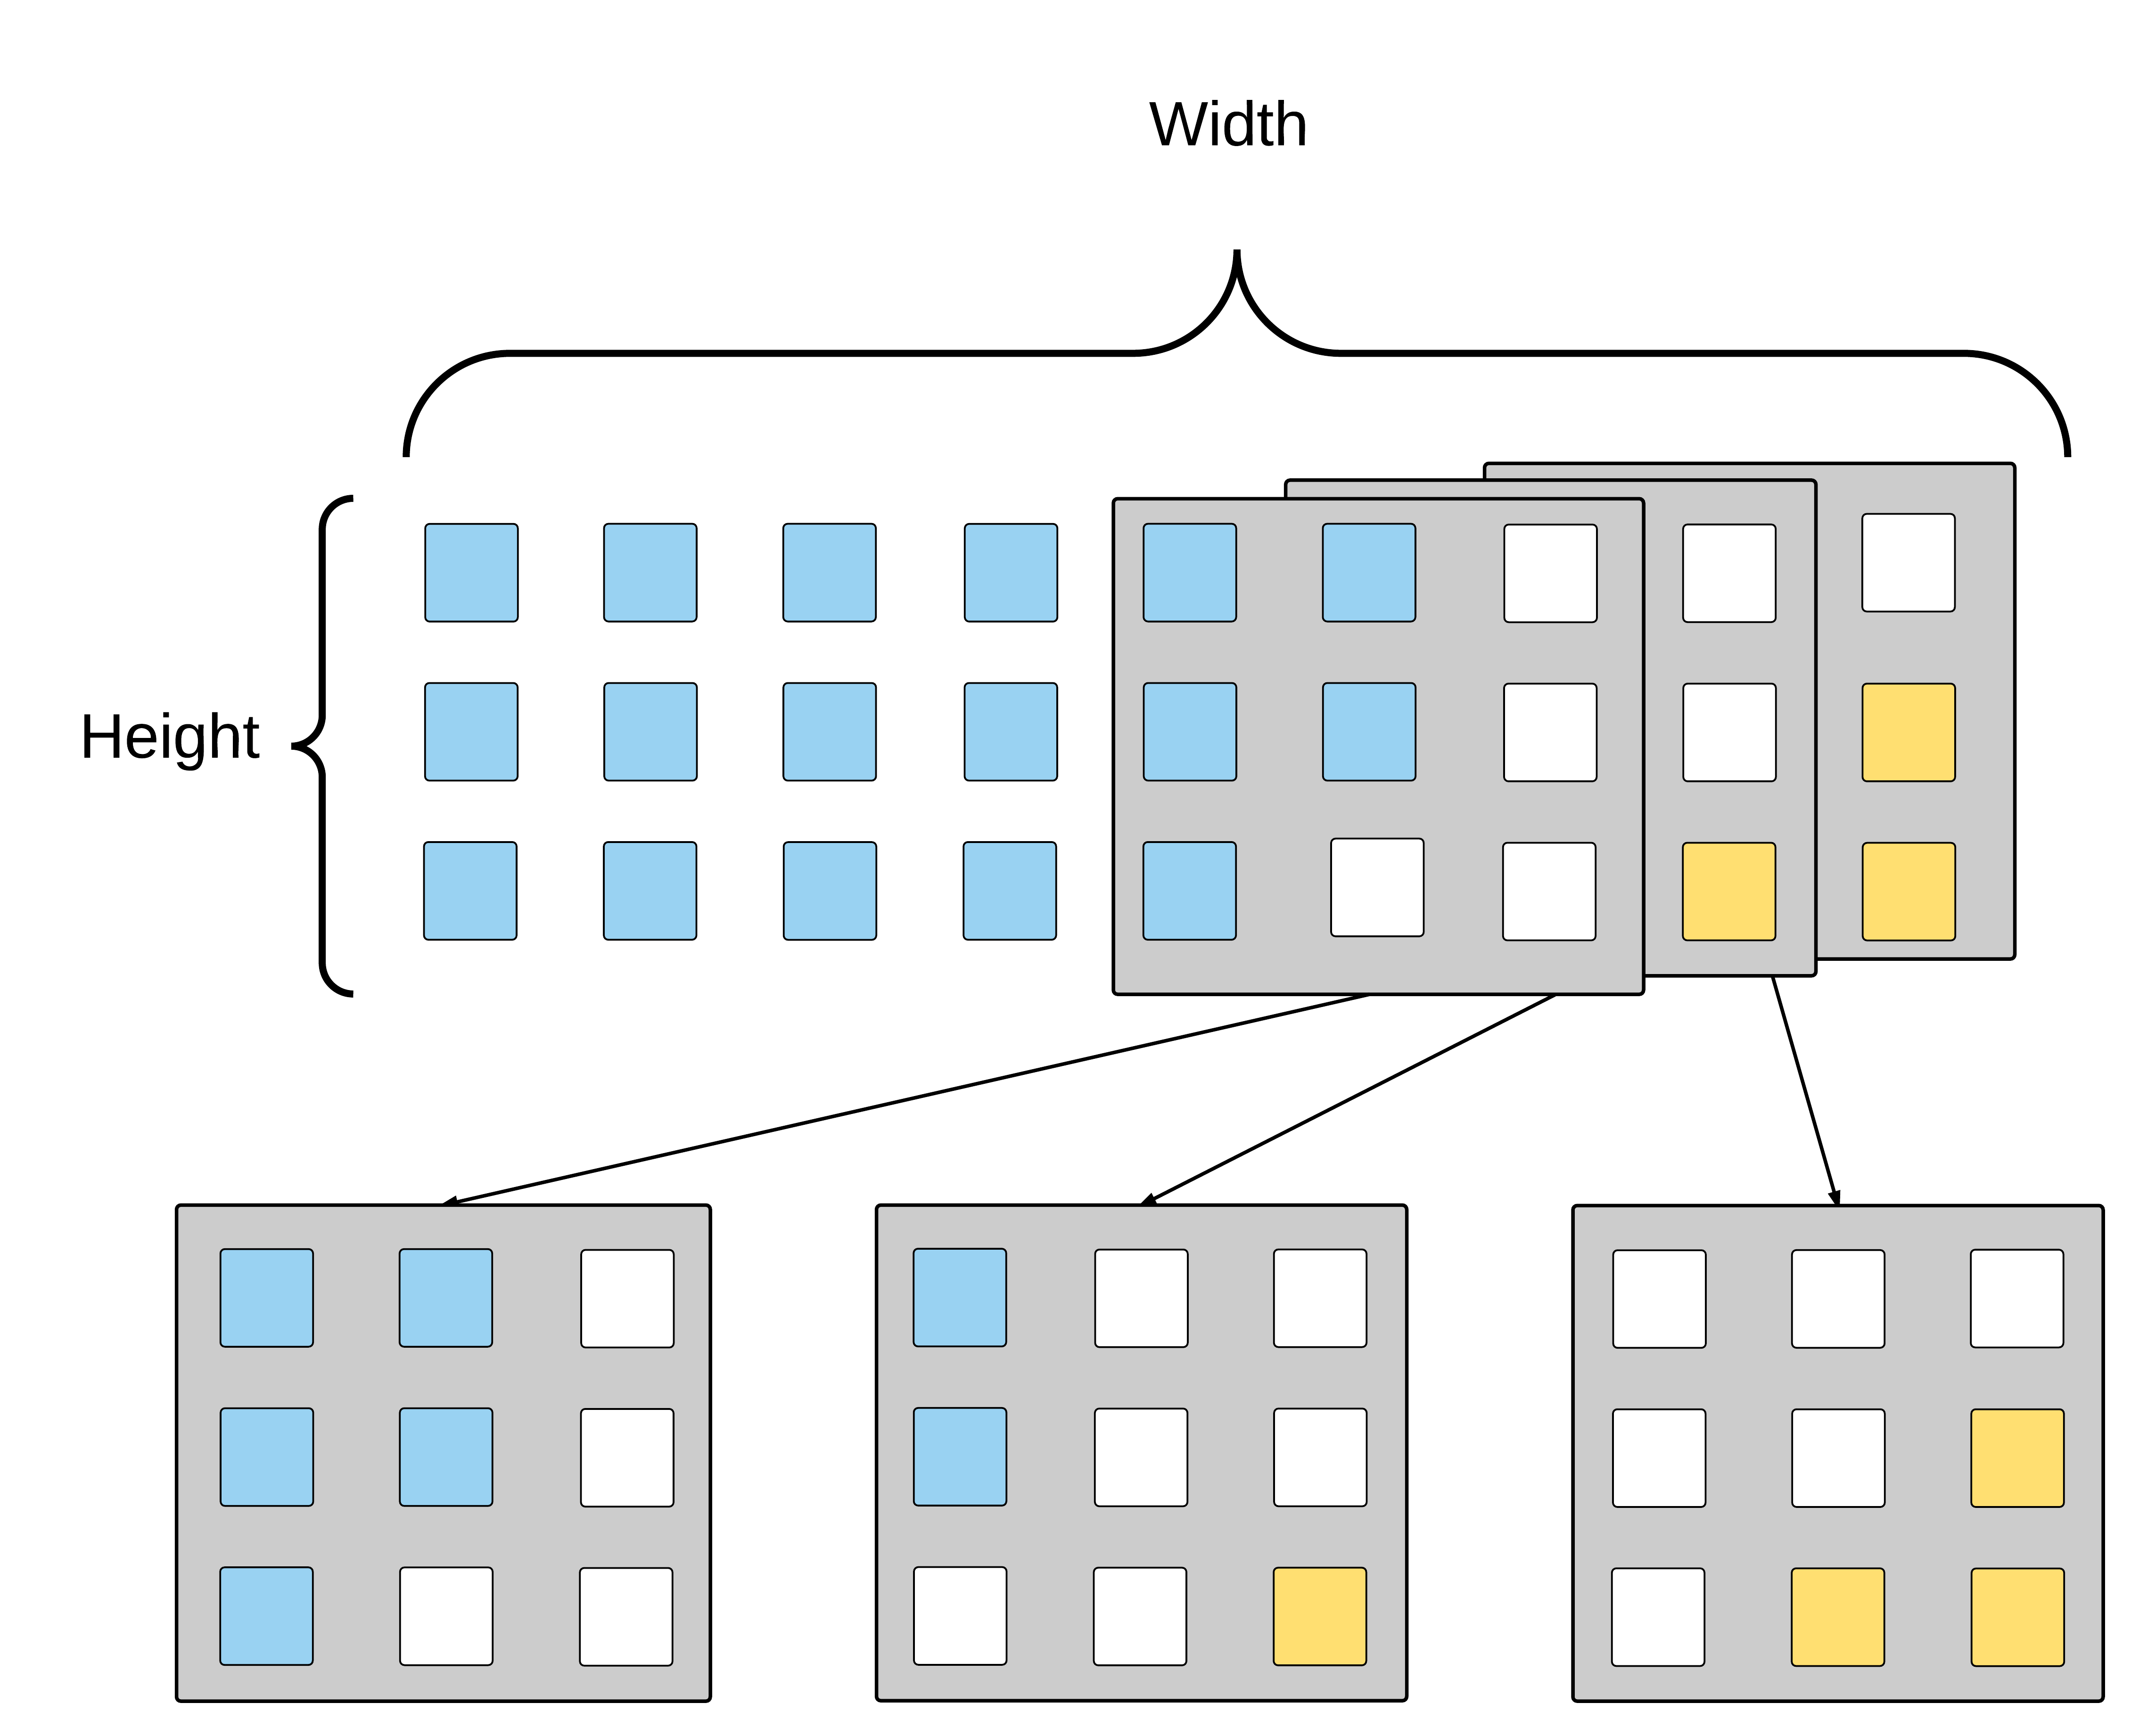
\includegraphics[width=10cm]{img/frontier1.png}
    \caption[The frontier.]{The frontier. The three rightmost pixels are shown with its full neighbourhood, which overlaps with its neighbours.}
    \label{fig:frontier1}
\end{figure}

\begin{figure}[h!]
    \centering
    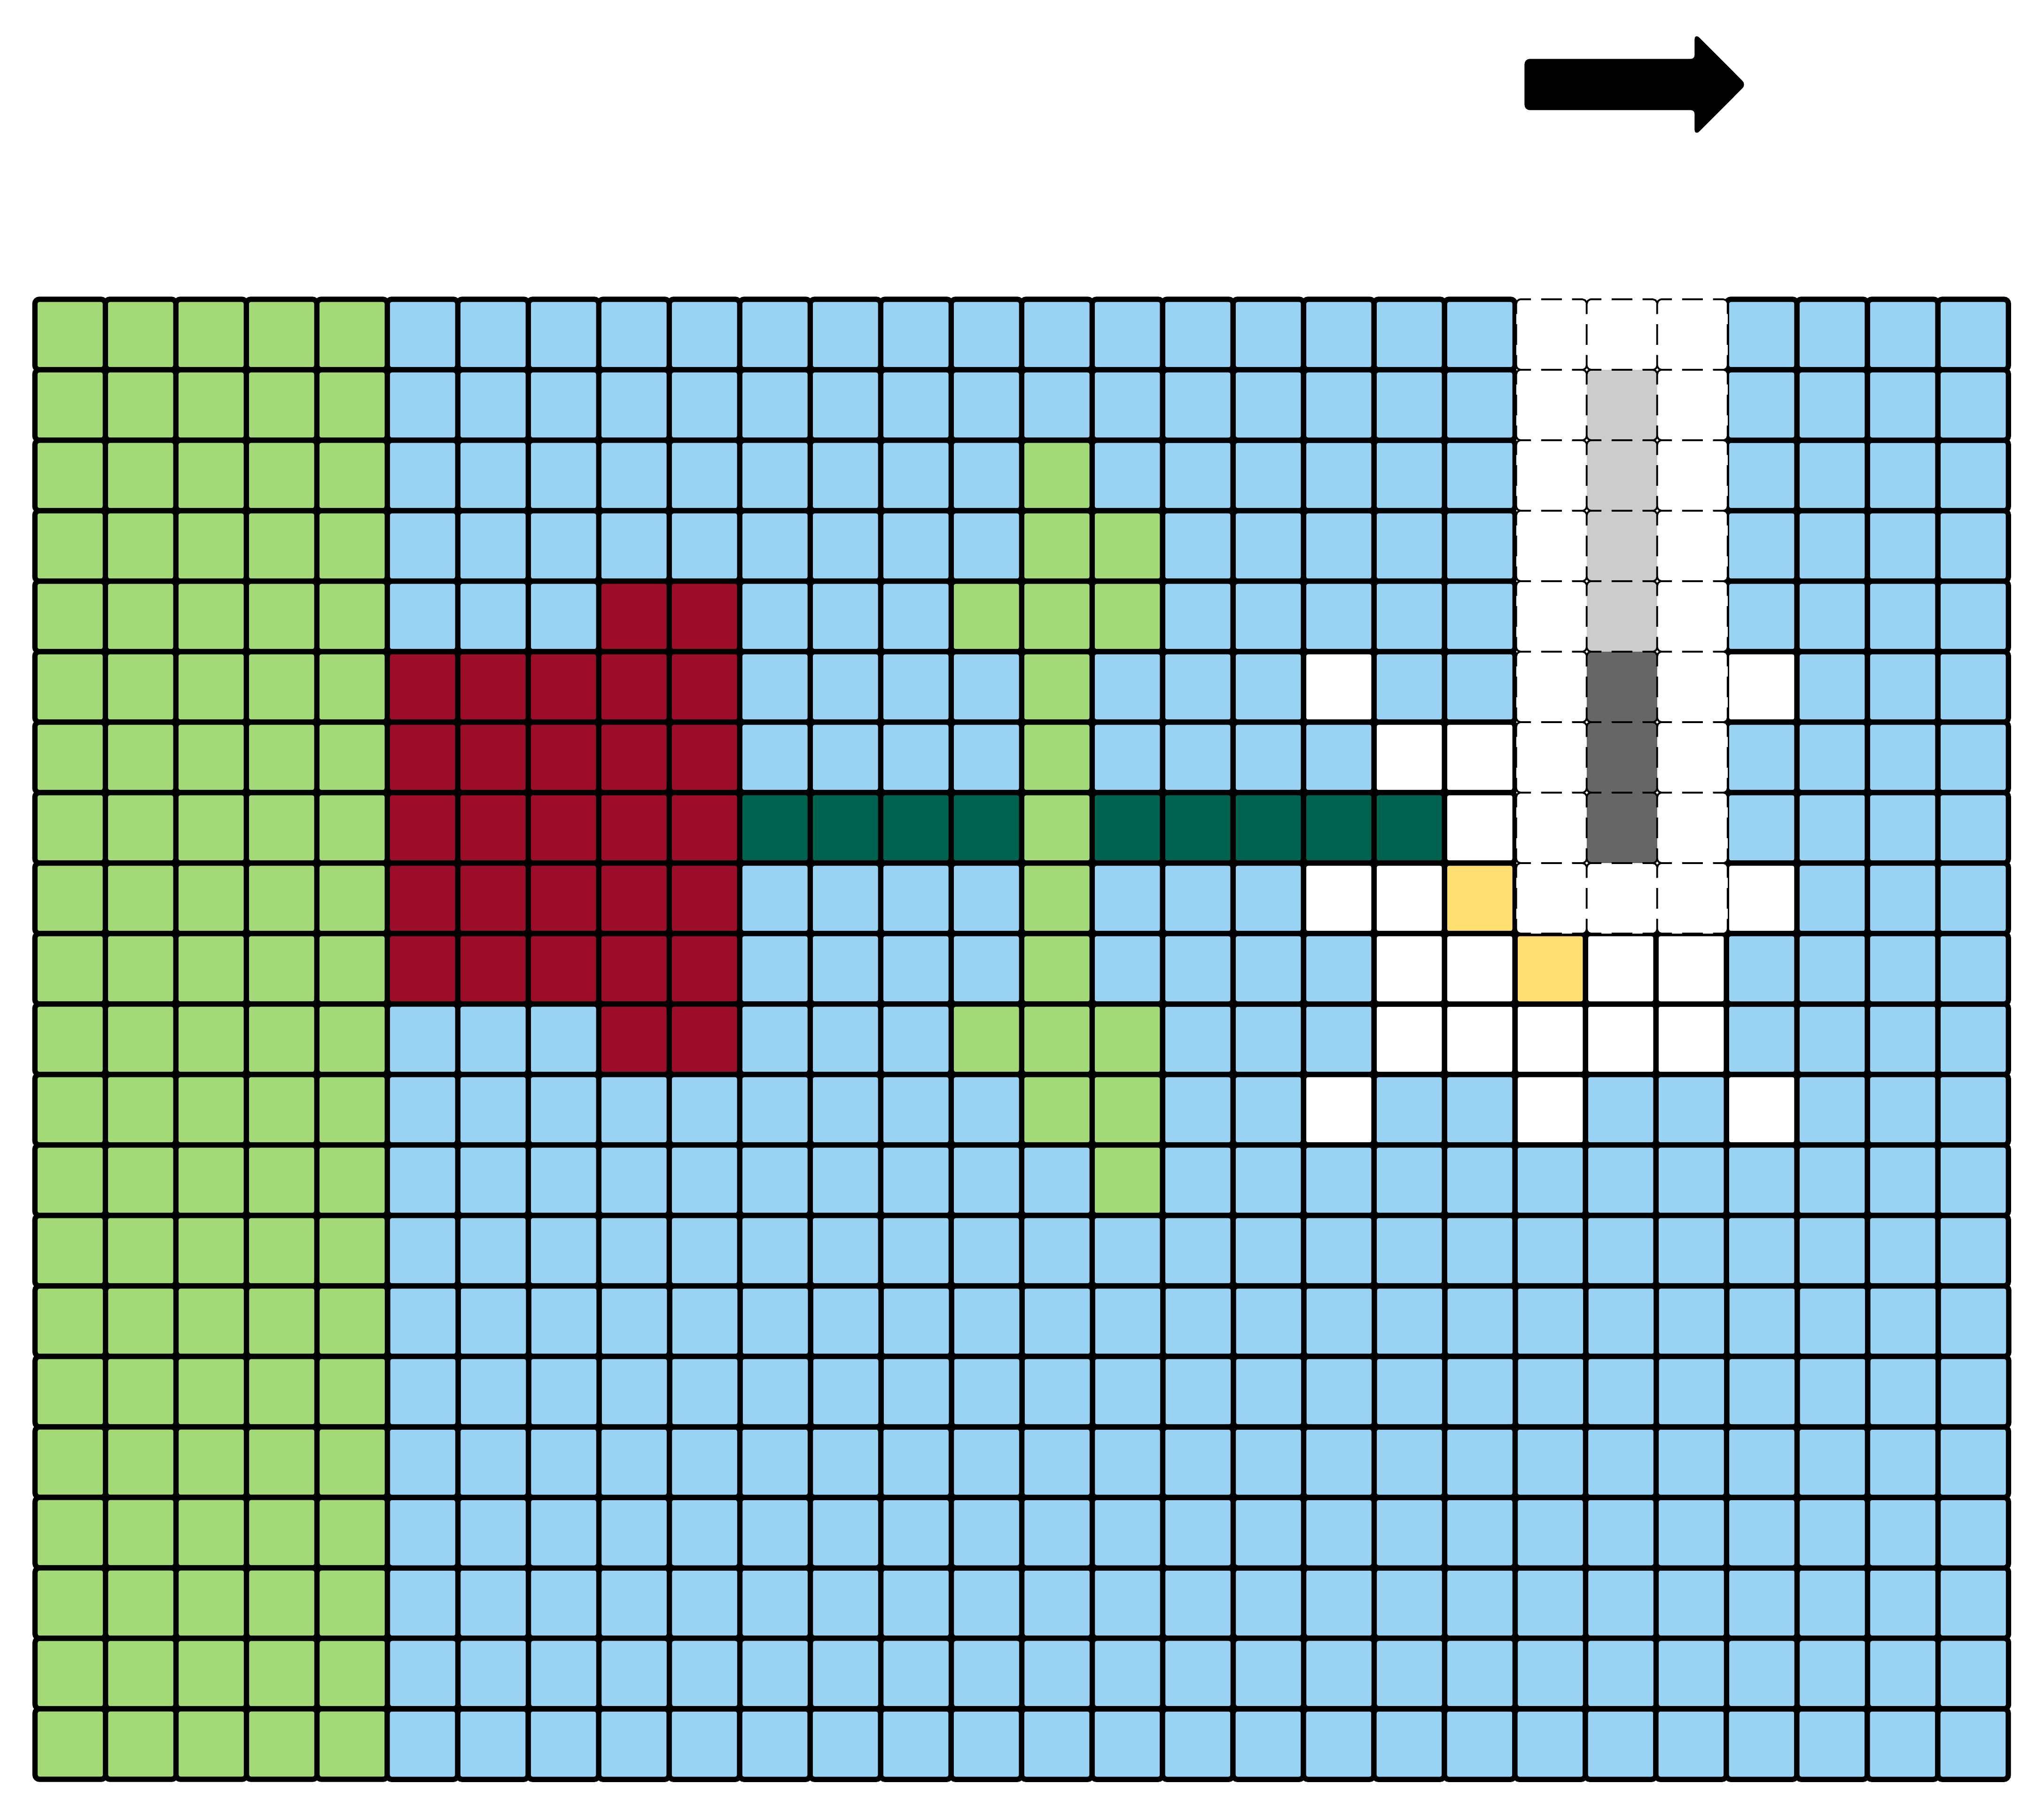
\includegraphics[width=10cm]{img/frontier2.png}
    \caption{The image from which the frontier in the previous figure is taken.}
    \label{fig:frontier2}
\end{figure}

